\section{Machine Learning}

When looking at artificial intelligence (AI), everything falls on a spectrum from easily explainable to being a black box when thinking about how the machine makes it's decisions.
On the easily explainable side of things, we have things like decision trees.

\begin{figure}[H]
  \centering
  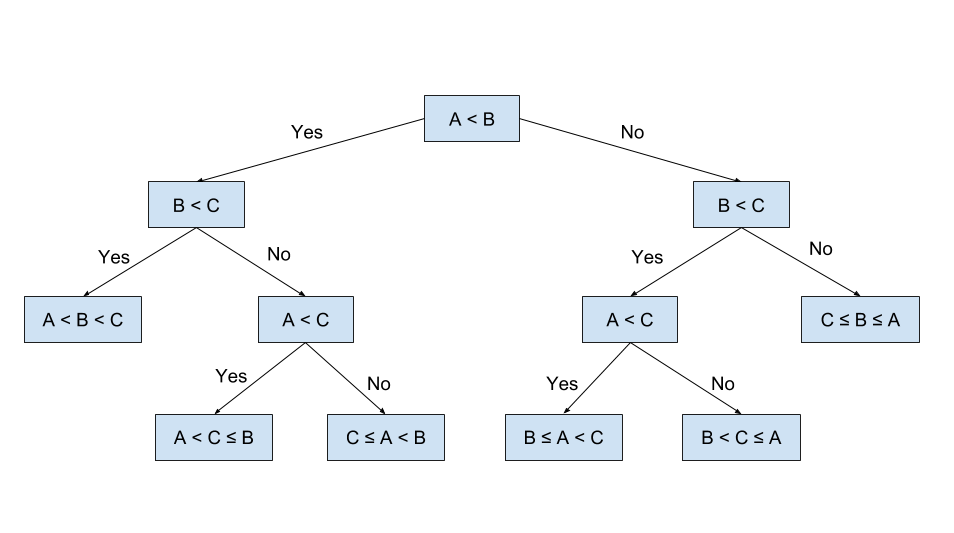
\includegraphics[width=120mm]{figures/decisionTree.png}
  \caption{Example of a basic decision tree}
  \label{decisionTree}
\end{figure}

A decision tree is where we sort the data by asking a sequence of questions and following the flowchart down to where it leads.
By the time we are at the bottom of the tree and have classified the data we can say exactly how the model does it's classification.
For instance if a decision tree is used for mortgage decisions and the model says no, we can query and learn that it said no because you had too low income or too low credit score for instance.

\begin{figure}[H]
  \centering
  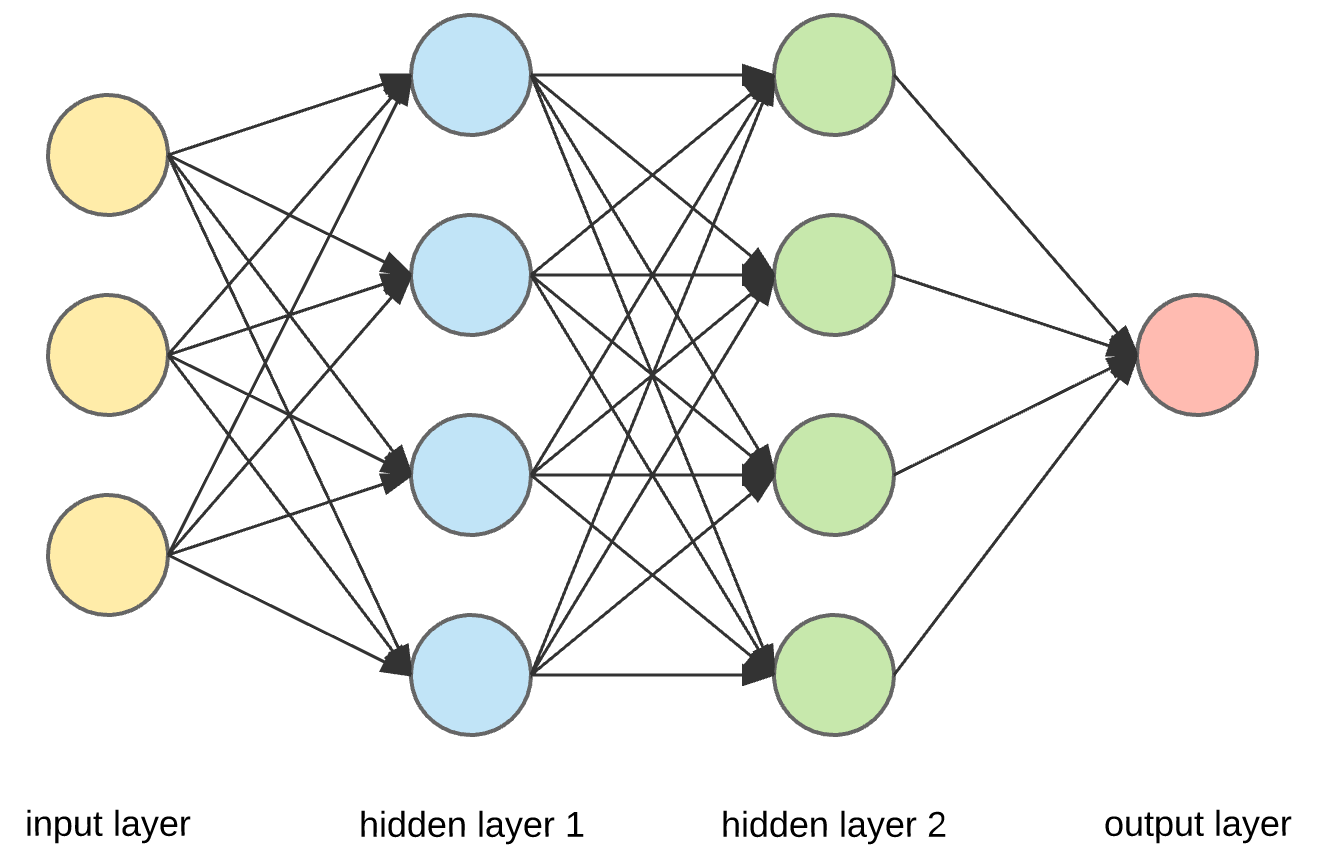
\includegraphics[width=120mm]{figures/neuralNet1.png}
  \caption{Example of a basic Neural Net}
  \label{neuralNet1}
\end{figure}

By contrast, a machine learning model like a neural net is almost a black box with regards to how the decisions are made.
We can query the model and ask it what it made its decisions based on, however, the features it picks out often isn't decipherable to humans in any way.
As in the previous example, if the answer to a mortgage is no, we have no real idea why the model made that decision.
That being said, neural networks are often able to come up with better outcomes for classification that simple models like decision trees are.
In the mortgage example, even if the neural net can't tell us how it comes to the conclusion of approving a loan, it is still more likely to be able to better tell who will be a good credit risk compared to the decision tree.
That's often the trade off that we make when deciding on a more opaque model.
That's why even though they are opaque in how they come up with their answers we still rely on them so heavily.
Because we can empirically test through monte-carlo studies how well they perform both in term of efficiency as well as how often these models misidentify the data that we are throwing at it.

While a neural network is opaque about how the decisions are made, the model itself doesn't have to be a black box for us.
We can take a peek under the hood and see how these models work.
To do so, we start up from the basic models like a perceptron and work our way to a graph neural network, finally connecting it to how neutrino reconstruction works.